\documentclass[a4paper, 11pt]{article}
%\documentclass[a4paper, 11pt, twoside, draft]{article}

%obecne
\usepackage[english]{babel}
\usepackage[utf8]{inputenc}

\usepackage[T1]{fontenc}


%Petr - pouzivam

%obecne
\usepackage[czech]{babel}
\usepackage[utf8]{inputenc}
%\usepackage[IL2]{fontenc}
\usepackage[T1]{fontenc}
% \usepackage{charter}



\usepackage{xspace}
\usepackage{framed}
\usepackage{mathtools}
\usepackage{pdflscape}
\usepackage[top=3cm, left=3.5cm, right=2.5cm, bottom=3cm, headheight=15pt, includeheadfoot]{geometry}%rozměry stránky
\usepackage{textcomp}
\usepackage{natbib}
\usepackage{hyperref}
\hypersetup{
    bookmarks=true,         % show bookmarks bar?
    unicode=false,          % non-Latin characters in Acrobat’s bookmarks
    pdftoolbar=true,        % show Acrobat’s toolbar?
    pdfmenubar=true,        % show Acrobat’s menu?
    pdffitwindow=false,     % window fit to page when opened
    pdfstartview={FitH},    % fits the width of the page to the window
    pdftitle={Smoderp manual},    % title
    pdfauthor={Kavka ...},     % author
    pdfsubject={Subject},   % subject of the document
    pdfcreator={Creator},   % creator of the document
    pdfproducer={Producer}, % producer of the document
    pdfkeywords={keyword1, key2, key3}, % list of keywords
    pdfnewwindow=true,      % links in new PDF window
    colorlinks=false,       % false: boxed links; true: colored links
    linkcolor=red,          % color of internal links (change box color with linkbordercolor)
    citecolor=green,        % color of links to bibliography
    filecolor=magenta,      % color of file links
    urlcolor=cyan           % color of external links
}
\usepackage[printonlyused]{acronym} %rejstik
% \usepackage{acronym} %rejstik
\makeatletter
\AtBeginDocument{%
  \renewcommand*{\AC@hyperlink}[2]{#2}%
}
\makeatother








% kvuli literature v htlatex
% \usepackage[nomain]{glossaries}
% \makeglossaries

%text
\usepackage{subcaption}
\captionsetup{compatibility=false}


\usepackage{listings} % inserting code 
\lstset
{ %Formatting for code in appendix
    language=Python,
    basicstyle=\footnotesize,
%     numbers=left,
%     stepnumber=1,
%     showstringspaces=false,
%     tabsize=1,
%     breaklines=true,
%     breakatwhitespace=true,
}


%tabulky
\usepackage{array}
\usepackage{tabulary}
\usepackage{multirow}
\usepackage{multicol}

%obrazky





% nuti obrazky aby nepretekali do dalsi sekce
\usepackage[section]{placeins}








%Lenka - nepouzivam
\usepackage{longtable}
\usepackage{siunitx}
\usepackage{rotating}
\usepackage[table,xcdraw]{xcolor}
\usepackage{booktabs}
\usepackage{url}
%\usepackage[pdftex,unicode,bookmarksnumbered,raiselinks=true]{hyperref}
% \usepackage{indentfirst}
\usepackage{fancyhdr}
\usepackage[font={footnotesize},labelfont=bf,justification=justified]{caption}
\usepackage{hhline}
\usepackage{colortbl}
\usepackage{array}
\usepackage{graphicx}

\usepackage{titlesec}



% \usepackage[table]{xcolor}
\usepackage{setspace}


% vetsi mezera mezi odstavci
\setlength{\parskip}{0.5em}


\usepackage{forest}    % na dir tree ale obecnejsi uziti
% \usepackage{indentfirst}

% tohle je jen prikaz na delatni popisu rovnic 
% jeho pouziti he v kapitole pouzite vztahy treba
\newcommand{\jj}[2]{
   & \acs{#1} & je \acl{#1}#2 \\
}




% kolek okolo cisla, pouzito v tabulce popisujici toolbox
\newcommand*\circled[1]{\tikz[baseline=(char.base)]{
            \node[shape=circle,draw,inner sep=2pt] (char) {{\scriptsize\sffamily#1}};}}



% Název smodepu 
% 
\newcommand{\smod}{SMODERP2D\xspace}


% upraveni casti
\titleformat
{\part} % command
[display] % shape
{\bfseries\Huge} % format
{Část \ \thepart\ } % label
{5ex} % sep
{
%     \rule{\textwidth}{1pt}
%     \vspace{1ex}
%     \centering
} % before-code
[
\vspace{-2.5ex}%
\rule{\textwidth}{0.3pt}
] % after-code
 
 
%%%% upraveni sekce
% \titlespacing*{\section}
% {0pt}{7.5ex}{2.5ex} 
 


% upraveni casti
\titleformat
{\part} % command
[display] % shape
{\bfseries\Huge} % format
{Part \ \thepart\ } % label
{5ex} % sep
{
%     \rule{\textwidth}{1pt}
%     \vspace{1ex}
%     \centering
} % before-code
[
\vspace{-2.5ex}%
\rule{\textwidth}{0.3pt}
] % after-code

% pokud toto odkomentujes
% \newcommand*{\DEBUG}{}
% zobrazi se poznamky
% poznamky jsou oznaceny @@@
%   
% prikaz na delani poznamek
\newcommand{\pozn}[1]{
   \ifdefined\DEBUG
   {\color{red}(@@@ #1)}
   \fi
}

\begin{document}

  \thispagestyle{empty}
  

\begin{titlepage} % Suppresses headers and footers on the title page

	\centering % Centre everything on the title page
	
	\scshape % Use small caps for all text on the title page
	
	\vspace*{\baselineskip} % White space at the top of the page
	
	%------------------------------------------------
	%	Title
	%------------------------------------------------
	
	\rule{\textwidth}{0pt}\vspace*{-\baselineskip}\vspace*{2pt} % Thick horizontal rule
	\rule{\textwidth}{0.4pt} % Thin horizontal rule
	
	\vspace{0.75\baselineskip} % Whitespace above the title
	
	{\LARGE \smod\ - Reference manual} % Title
	
	\vspace{0.75\baselineskip} % Whitespace below the title
	
	\rule{\textwidth}{0.4pt}\vspace*{-\baselineskip}\vspace{3.2pt} % Thin horizontal rule
	\rule{\textwidth}{0pt} % Thick horizontal rule
	
	\vspace{2\baselineskip} % Whitespace after the title block
	
	%------------------------------------------------
	%	Subtitle
	%------------------------------------------------
	
	Simulation model of overland flow and erosion processes
	
	\vspace*{3\baselineskip} % Whitespace under the subtitle
	
	%------------------------------------------------
	%	Editor(s)
	%------------------------------------------------
	
	Edited By
	
	\vspace{0.5\baselineskip} % Whitespace before the editors
	
	{\scshape\Large Kavka, Jeřábek, Landa, Pešek \\ ... \\} % Editor list
	
	\vspace{0.5\baselineskip} % Whitespace below the editor list
	
	\textit{CTU in Prague} % Editor affiliation
	
	\vfill % Whitespace between editor names and publisher logo
	
	%------------------------------------------------
	%	Publisher
	%------------------------------------------------
% 	
\includegraphics[width=0.5\textwidth]{./img/logo.png}
	
	
	
	\begin{verbatim}
    @ @ @   @       @     @ @     @ @ @     @ @ @ @  @ @ @    @ @ @
   @        @ @   @ @   @     @   @     @   @        @     @  @     @
   @        @   @   @  @       @  @      @  @        @     @  @     @
     @ @    @       @  @       @  @      @  @ @ @    @ @ @    @ @ @
         @  @       @  @       @  @      @  @        @   @    @
         @  @       @   @     @   @     @   @        @    @   @
    @ @ @   @       @     @ @     @ @ @     @ @ @ @  @     @  @

   \  \  /   / /    \   \  /   \  /    /     /        @ @ @   @ @ @
    \ _\/   /_/      \   \/     \/    /_____/        @     @  @     @
        \__/          \  /      _\___/                     @  @      @
            \____      \/      /                          @   @      @
                 \_____/______/                         @     @      @
                              \                       @       @     @
                               \____________________ @ @ @ @  @ @ @
 \end{verbatim}
 
 
 
% 	\plogo % Publisher logo
        
	
	\vspace{0.3\baselineskip} % Whitespace under the publisher logo
	
	2024 % Publication year
	
	{\large publisher} % Publisher

\end{titlepage}

%----------------------------------------------------------------------------------------




  \newpage
  \pagenumbering{roman}
  \setcounter{page}{1} % obsah a seznamy skratek, obrazku a tabulek rimska cislice od i
  \tableofcontents\addcontentsline{toc}{section}{Obsah}

  \newpage
  \pagenumbering{arabic}\setcounter{page}{1}% od uvodu do konce arabske cislice od 1
  \part{Introduction}
  

\section{Introduction and model overview}

%!TEX ROOT = ../manual_CZ.tex


Dostává se Vám do ruky uživatelský manuál modelu \smod. Celý název modelu je: Simulační Model Povrchového Odtoku a Erozního Procesu. Tento model lze využít pro výpočet hydrologicko erozních procesů na jednotlivých pozemcích nebo na malých povodích. Výstupy z modelu jsou primárně určeny pro stanovení odtokových poměrů v ploše povodí a parametrů opatření pro snížení odtoku z povodí a erozního ohrožení zemědělské půdy. Model lze využít při navrhování komplexnějších soustav sběrných a odváděcích prvků nebo suchých nádrží a polderů. Jeho využití předpokládají jak současné metodiky, tak i technické normy a doporučené standardy.
Z hlediska kategorizace se jedná o fyzikálně založený plně distribuovaný dvourozměrný epizodní model. 
% 
Nově zavedené prostorové řešení (2D), které nahradilo dřívější profilovou verzi modelu, umožňuje komplexní řešení a náhled na celou řešenou lokalitu a přesnější popis zpravidla heterogenní morfologie zemského povrchu. 
% 
Přechod modelu na 2D řešení umožňuje zejména větší dostupnost potřebných dat a zvyšující se kapacita výpočetní techniky. 
% 
% Přesto, že dvourozměrné řešení je z hlediska vstupních dat a vnitřních procesů složitější, nicméně benefity distribuovaného řešení převažují. 
% Dostupnost vstupních dat v podrobném rozlišení se zlepšuje, stejně tak jako se zvyšuje výpočetní kapacita výpočetní techniky.
% 
% 
Vývoj modelu je podporován z veřejných prostředků a podílejí se na něm studenti a zaměstnanci Katedry hydromeliorací a krajinného inženýrství Fakulty stavební ČVUT v Praze.
Pro snazší orientaci je manuál rozdělen na dvou hlavních částí. 
% 
V první části jsou uvedeny zvolené výpočetní vztahy pro popis povrchového odtoku. 
% 
Druhá část je věnována popisu instalace a použití modelu v prostředí ArcGIS. Dále jsou zde podrobně popsána vstupní a výstupní data a stručně popsán tok programu. 
% Ve třetí části jsou ukázány výsledky z řečení konkrétní lokality.
Případné aktualizace, vzorová data, ukázky využití a další informace o modelu \smod jsou průběžně poskytovány na webových stránkách (\href{http://storm.fsv.cvut.cz/cinnost-katedry/volne-stazitelne-vysledky/smoderp/?lang=cz}{storm.fsv.cvut.cz/cinnost-katedry/volne-stazitelne-vysledky/smoderp/}).


\subsection*{Hydrologické modelování}\addcontentsline{toc}{subsection}{Hydrologické modelování}
Hydrologické modelování s využitím geografických informačních sytému (GIS) je oblast vyvíjející se od konce 70. let. Hydrologické modelu využívaly (a využívají) technologii operací s geodaty a databázemi, které GIS umožňuje. Přesto jsou některé topologické operace pro hydrologické modely specifické (např. definice rozvodnice povodí, lokalizace/odstranění bezodtokových míst)~\citep{devantier1993}. V zásadě se rozvíjeli modelu povrchového odtoku založené na pravidelném rastru, nepravidelné trojúhelníkové síťi (TIN) nebo na vrstevnisích (contour-based)~\citep{devantier1993}. Rovněž docházelo k vývoji celistvých~\footnote{povodí je rozděleno na sub-povodí která jsou řešena celistvě například metodou SCS křivek} nebo plně distribuovaných modelů~\citep{devantier1993}. S vývojem informační techniky docházelo k větší integraci GIS softwaru a hydrologických modelů. Na obrázku~\ref{fig:klasGISHyd} je ukázána klasifikace propojení GIS a hydrologických modelu na konci 90. let~\citep{sui1999}. Hydrologický model buďto pouze využívá některé funkcionality GIS softwaru (obrázek~\ref{fig:klasGISHyd}a). V opačném případě již vývojář GIS softwaru integruje do systému některé prvky hydrologických modelů (obrázek~\ref{fig:klasGISHyd}b). GIS software a hydrologické model si pouze vyměňují některá data (pomocí binárních nebo ascii souborů (obrázek~\ref{fig:klasGISHyd}c), nebo GIS software umožňuje ve svém prostření vložit uživatelem vytvořené skripty, která pak tvoří hydrologický model (obrázek~\ref{fig:klasGISHyd}b)\footnote{Toto je případ modelu SMODERP2D pokud je spouštěn v prostředí ArcGIS}~\citep{sui1999}. Autoři studie se k těmto postupů staví kriticky. Jejich základní výhradou je, že struktury GIS software vytvářejí bariery pro popis hydrologických dějů, které mají jistá specifika. Konceptualizace pomocí vrstev ať už rastrových  nebo vektorových nemusí vyjadřovat heterogenitu hydrologických dějů nebo užití stochastických modelů. GIS softwary často umožňují pouze limitovanou prací časové proměnlivými ději~\citep{sui1999}.

\begin{figure}
  \centering
  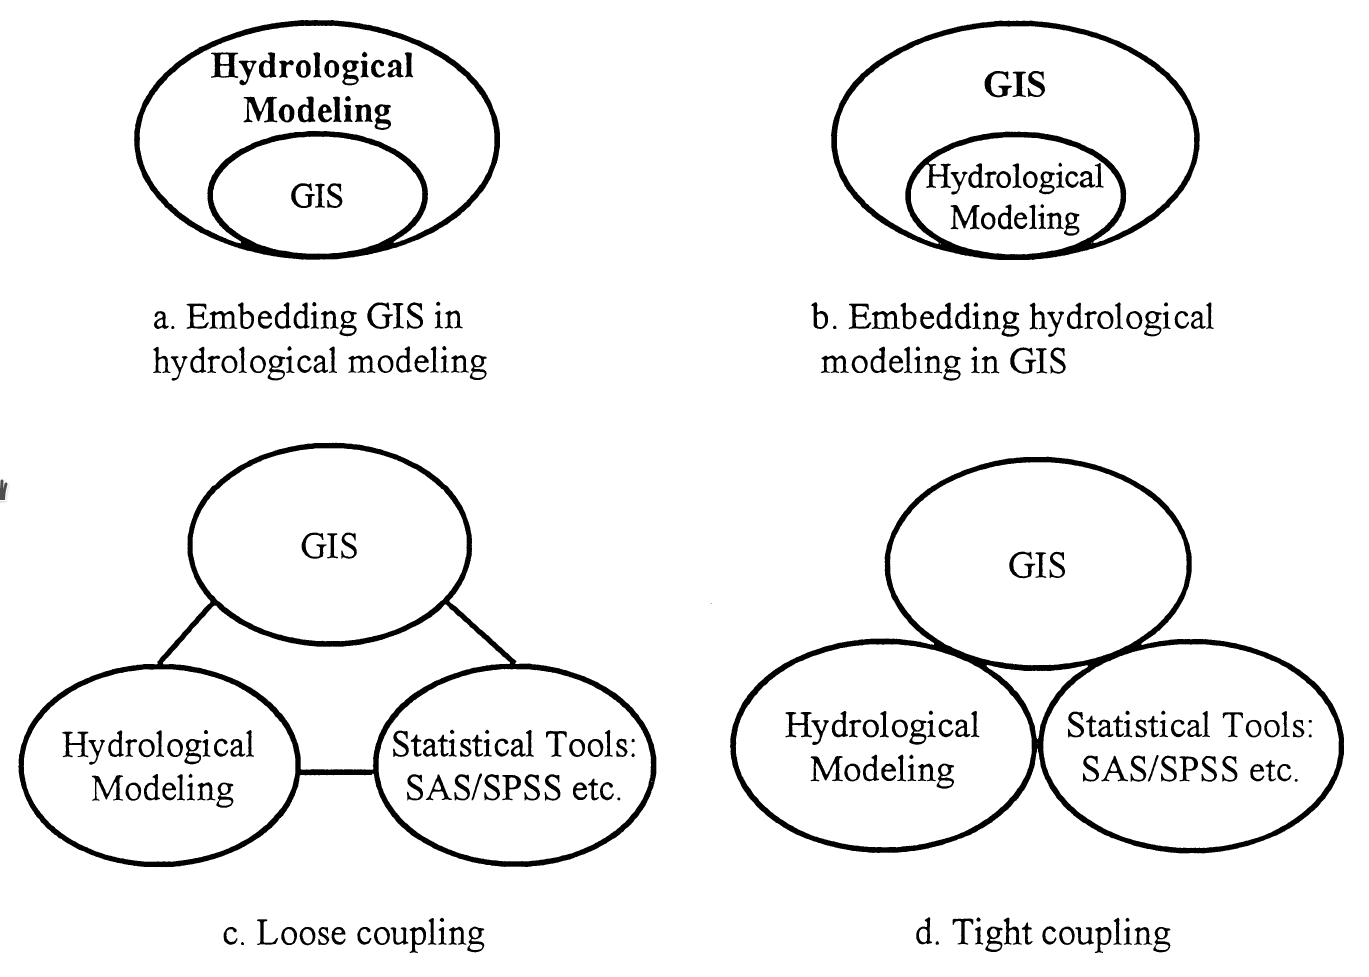
\includegraphics[width=\linewidth]{./img/klasifikaceGISHyd.png}
  \caption{Klasifikace integrace hydrologických modelu podle~\cite{sui1999}}
  \label{fig:klasGISHyd}
\end{figure}

Při popisu povrchového odtoku se nejčastěji využívá jedno ze zjednodušení Saint-Venantových (SV) rovnic ať už kinematickou nebo difuzní. 
\pozn{Diffuzni vlna zjednodušuje SV rovnice tím, že zanedbava člen konvekčního zrychlení (setrvacnost) (Chaudhry, 1993). pochopit a doplnit}
Příklad řešení povrchového odtoku pomocí kinematickou například: \cite{taylor1974} nebo \cite{goodrich1991}. V případě druhé studie bylo 2D řešení kinematické vlny řešeno pro jednotlivé trojúhelníky TIN sítě. Celkový odtok byl pak výpočtem 1D routingem odtoku z jednotlivých trojúhelníků TIN sítě. Kinematická vlna pro řešení povrchového odtoku je implementována například v modelu HEC-1~\citep{macarthur1993}. Jako příklad řešení povrchového odtoku pomocí difuzní vlny může být například~\cite{julien1995}, kde byla rovněž implementována prostorově distribuovaná srážka vhodná pro řešení bleskových povodí v aridních oblastech. V \cite{jain2004} bylo směrování odtoku definované pomocí jednosměrného algoritmu D8, samotný byla ale řešen pomocé difuzní vlny. Jako příklady softwaru, kde byla využita difuzní vlna k řešení povrchového odtoku je například: SHE~\cite{abbott1986_1, abbott1986_2}, CAS2D~\cite{julien1995}, WEPP~\citep{flanagan2010} nebo SWAT ~\citep{USDA}. V literatuře lze rovněž najít kritéria na základě kterých lze určit vhodnost obou řešení~\cite{singh1994, moramarco2002}

V modelech obecně je třeba dobře zvolit časovou a prostorovou diskretizaci.  U řešení povrchového odtoku byly zjištěny problémy s časovou diskretizací, kde docházelo k nestabilitám i při dodržení Courant–Friedrichs–Lewiho kritéria. To je způsobeno zejména malou hloubkou hladiny na povrchů vůči velikosti buňky rastru, drsnostnímu koeficientu nebo změně sklonu mezi sousedícími buňkamiA~\cite{zhang1989, esteves2000}. V \cite{molnar2000} byl studován vliv velikosti buňky rastru na výsledek modlu povrchového odtoku. Různá velikost buněk v rastru příliš neovlivňovala výsledné řešení pokud byla kalibrace provedena na rastru se stejně velkou buňkou. U řešení s větší buňkou bylo na povodí větší oblast, kde vznikl povrchový odtok a po kalibraci byla větší drsnost koryt hydrografické sítě.









\section{Rainfall data}

\section{Hillslope hydrology and hydraulics}

    \subsection{Water balance (JJ)}

    The SMODERP2D episodic rainfall-runoff/erosion model was used for the
    investigation presented here. The 2D model is based on a 1D profile version, in
    which the surface runoff and the erosion were typically calculated in several
    1D profiles representing the main flow path in the hillslope \cite{Dostal2000}.
    The current generation of the SMODERP2D model is pixel distributed, and is
    implemented in python in order to be compatible with most GIS software. The
    development is presented on the github platform at
    \href{https://github.com/storm-fsv-cvut/smoderp2d}{github.com/storm-fsv-cvut/smoderp2d}.

    The SMODERP2D model is primarily designed for surface runoff and erosion
    computation. The surface flow routing in the model is based on the digital
    elevation model (DEM). DEM also controls the spatial discretization of the
    model. The principle of the model is the cell-by-cell mass balance calculated
    in each time step. The change in the water level of the shear flow in any cell
    in time is controlled using the equation: 
    \begin{equation} 
    \frac{\mathrm{d}h}{\mathrm{d}t} = es_{i,t-1} + q^{in}_{i,t-1} - inf_{i,t-1} - q^{out}_{i,t-1},
    \label{eq:bilance}
    \end{equation}
    where h is the surface water level (L), qin and qout are the sheet overland
    inflow and outflow into and out of a given raster cell ($\mathrm{L.t^{-1}}$),
    ep is the effective precipitation intensity (the potential precipitation
    reduced by the interception zone and the surface retention)
    ($\mathrm{L.t^{-1}}$), and inf is the infiltration rate ($\mathrm{L.t^{-1}}$).
    The kinematic wave approach is used in the calculation of the overland flow.
    The momentum is therefore expressed by the power-law:

    \begin{equation} 
    q = ah^b
    \label{eq:powerlaw}
    \end{equation}
    where a and b are power-law parameters. Equation \ref{eq:powerlaw} can be
    expressed in the form of the Manning–Strickler formula


    \begin{equation} 
    q = n^{-1} s^Y h^b,
    \label{eq:powerlaw}
    \end{equation}
    where n is roughness,  Y  empirical parameter and s is the surface slope ($\mathrm{L.L^{-1}}$).

    The infiltration component of Equation \ref{eq:bilance} is calculated by the
    Philip infiltration equation \citep{philip1957}
    \begin{equation} 
    inf = \frac{1}{2}St^{-1/2}+K_s.
    \label{eq:infiltration}
    \end{equation} 

    where S stands for sorptivity ($\mathrm{L.t^{1/2}}$) and ($\mathrm{K_s}$)
    stands for saturation hydraulic conductivity ($\mathrm{L.t^{-1}}$).

    The SMODERP2D model is subjected to uniform rainfall. The potential
    precipitation is reduced due to surface retention. The surface retention is the
    storage that needs to be filled before surface runoff can occur. 

    The flow routing of the surface runoff is based on the D8 one-direction flow
    algorithm \cite{o1984extraction}. The inflow to cell i is defined as the sum of the sheet
    outflows from the adjacent cells, as:

    \begin{equation} 
    q^{in}_{i,t-1} = \sum_j^m q^{out}_{j,t-1}, 
    \label{eq:d8}
    \end{equation} 
    where j is the index of the adjacent up-slope cells identified by the D8 flow
    algorithm.

    The time derivative in Equation \ref{eq:bilance} is calculated using an
    explicit method. The computation is therefore sensitive to the size of the time
    step. The size of the time step is controlled by the Courant criterion, which
    needs to be kept below the theoretical maximum value of 1, while the maximum
    value in practise is lower than 1 
    \cite{zhang1989modeling, esteves2000overland}.


    The sheet flow water level of the next time t + 1 step in Equation
    \ref{eq:bilance} which incorporates the sum \ref{eq:d8} is calculated with the
    explicit time discretisation scheme for cell i as:
    \begin{equation} 
    h_{i,t} =h_{i,t} + \mathrm{d}t (es_{i,t-1} + \sum_j^m q^{out}_{j,t-1}-
    inf_{i,t-1} - q^{out}_{i,t-1}),
    \label{eq:bilance}
    \end{equation}

    %The principle of the model is the cell-by-cell mass balance calculated in each
    %time step. The change in the water level of the shear flow in any cell in time
    %is controlled using the equation:  
    %
    %[Equation] 
    %	
    %(1) 
    %
    %where h is the surface water level (L), qin and qout are the sheet overland
    %inflow and outflow into and out of a given raster cell (L.t−1), ep is the
    %effective precipitation intensity (the potential precipitation reduced by the
    %interception zone and the surface retention) (L.t−1), and inf is the
    %infiltration rate (L.t−1).  
    %
    %The SMODERP2D model is subjected to uniform rainfall. The potential
    %precipitation is reduced due to surface retention. The surface retention is the
    %storage that needs to be filled before surface runoff can occur.  
    %
    %The time derivative in Equation (1) is calculated using an explicit method. The
    %computation is therefore sensitive to the size of the time step. The size of
    %the time step is controlled by the Courant criterion, which needs to be kept
    %below the theoretical maximum value of 1, while the maximum value in practise
    %is lower than 1 [46,47].  
    %
    %The sheet flow water level of the next time t + 1 step in Equation (1) which
    %incorporates the sum (5) is calculated with the explicit time discretisation
    %scheme for cell i as: 
    %
    %[Equation] 
    %	
    %(6) 

        \subsubsection{Interception component (JJ)}
        \subsubsection{Infiltration component (JJ) }

 
            %Phillip infiltration 
            %
            %The infiltration component of Equation (1) is calculated by the Philip infiltration equation [44] 
            %
            %[Equation], 
            %	
            %
            %(4) 
            %
            %where S stands for sorptivity (L.t1/2) and Ks stands for saturation hydraulic conductivity (L.t−1). 
            %
            %GA??? 

 

        \subsubsection{Surface retention component (JJ)}
    \subsection{Sheet flow hydraulics (JJ)}
        \subsubsection{Principle of the solution}

             %The kinematic wave approach is used in the calculation of the overland flow. The momentum is therefore expressed by the power-law: 
             %
             %[Equation], 
             %	
             %
             %(2) 
             %
             %where a and b are power-law parameters. Equation (2) can be expressed in the form of the Manning–Strickler formula 
             %
             %[Equation] 
             %	
             %
             %(3) 
             %
             %where b and Y are empirical parameters and s is the surface slope (L.L−1). n- Manning roughness coefficient for sheet flow 
             %
             % 
             %
             %XXX -  tables here or link to user guide 

        \subsubsection{D8/ Multiple flow approach}

            %Two (optional) types of flow direction can be used in the model solution 
            %
            %D8 algorithm 
            %
            %The flow routing of the surface runoff is based on the D8 one-direction flow algorithm [45]. The inflow to cell i is defined as the sum of the sheet outflows from the adjacent cells, as: 
            %
            %[Equation], 
            %	
            %
            %(5) 
            %
            %where j is the index of the adjacent up-slope cells identified by the D8 flow algorithm. 
            %
            %Multiple flouw algorithm 
            %
 

        \subsection{Rill flow formation and hydraulics (JJ)}

            The rill flow is also included in the calculation. In SMODERP2D, rill flow in a
            cell occurs if $h>h_{crit}$, where $h_{crit}$ is the critical water level. The
            water flow corresponding to the water level above the critical water level has
            enough energy to start to carry the soil particles and to create a rill.

            The critical water level $h_{crit}$ is calculated as:
            \begin{equation}
              h_{crit} = MIN(h_{v_{crit}},h_{\tau_{crit}}),
              \label{eq:critdef}
            \end{equation}
            where $h_{v_{crit}}$ is the water corresponding to the critical velocity, and
            $h_{\tau_{crit}}$ is the water level corresponding to the critical shear
            stress.  As shown in Formula \ref{eq:critdef}, $h_{crit}$ uses several values
            obtained with a different approach. This approach is adopted in order to remain
            on the safe side of the emergence of a rill, since $h_{v_{crit}}$ is more
            sensitive to the sheet flow velocity and $h_{\tau_{crit}}$ is more sensitive to
            the slope of the soil surface. 

            When the condition $h>h_{crit}$ is fulfilled, a rill starts to develop in a
            given cell and $h_{sheet}=h_{crit}$. In SMODERP2D, the rill is a dynamic component and
            can increase as the rill flow increases. The rill volume is controlled by the
            volume of water corresponding to the rill water level $h_{rill}$. This volume is
            calculated as:


            \begin{equation}
              V_{rill} = h_{rill}P,
              \label{eq:rillvol}
            \end{equation}

            The critical water level $h_{crit}$ is calculated as:
            \begin{equation}
              h_{rill} = MAX(h-h_{crit},0),
              \label{eq:hrill}
            \end{equation}
            P stands for the size of the raster cell. The rill is simplified as a small
            channel at the soil surface with a rectangular cross section. The rectangle has
            width $b_{rill}$ and rill height $y_{rill} = 0.7b_{rill}$. The rill flow is as
            calculated with the Manning equation: 

            \begin{equation}
                q_{rill} = \frac{A}{n_{rill}} s^{1/2} R_{rill}^{2/3},
              \label{eq:rillflow}
            \end{equation}
            where A is the cross section of the rill,  $n_{rill}$ is the roughness in the
            rill, s is the surface slope, and  $R_{rill}$  is the hydraulic radius of the
            rill. 

            As stated above, the size of the rill changes as $h_{rill}$ increases. The
            scheme of this change is shown in Figure \ref{fig:rill_plneni}. The change in
            the rill flow varies with the change in $R_{rill}$ in Equation
            \ref{eq:rillflow}, since $h_{rill}$ increases, and therefore $y_{rill}$ and
            $b_{rill}$ also increase. The $R_{rill}$ for an increasing rill is calculated
            as:
            \begin{equation}
                R_{rill} = \frac{h_{rill}b_{rill}}{2h_{rill}+b_{rill}}  =
                \frac{y_{rill}b_{rill}}{2y_{rill}+b_{rill}},
              \label{eq:rrill}
            \end{equation}
            where:
            \begin{equation}
              b_{rill} = h_{rill}/0.7
              \label{eq:brill}
            \end{equation}


            \begin{figure}[b]
                \centering
                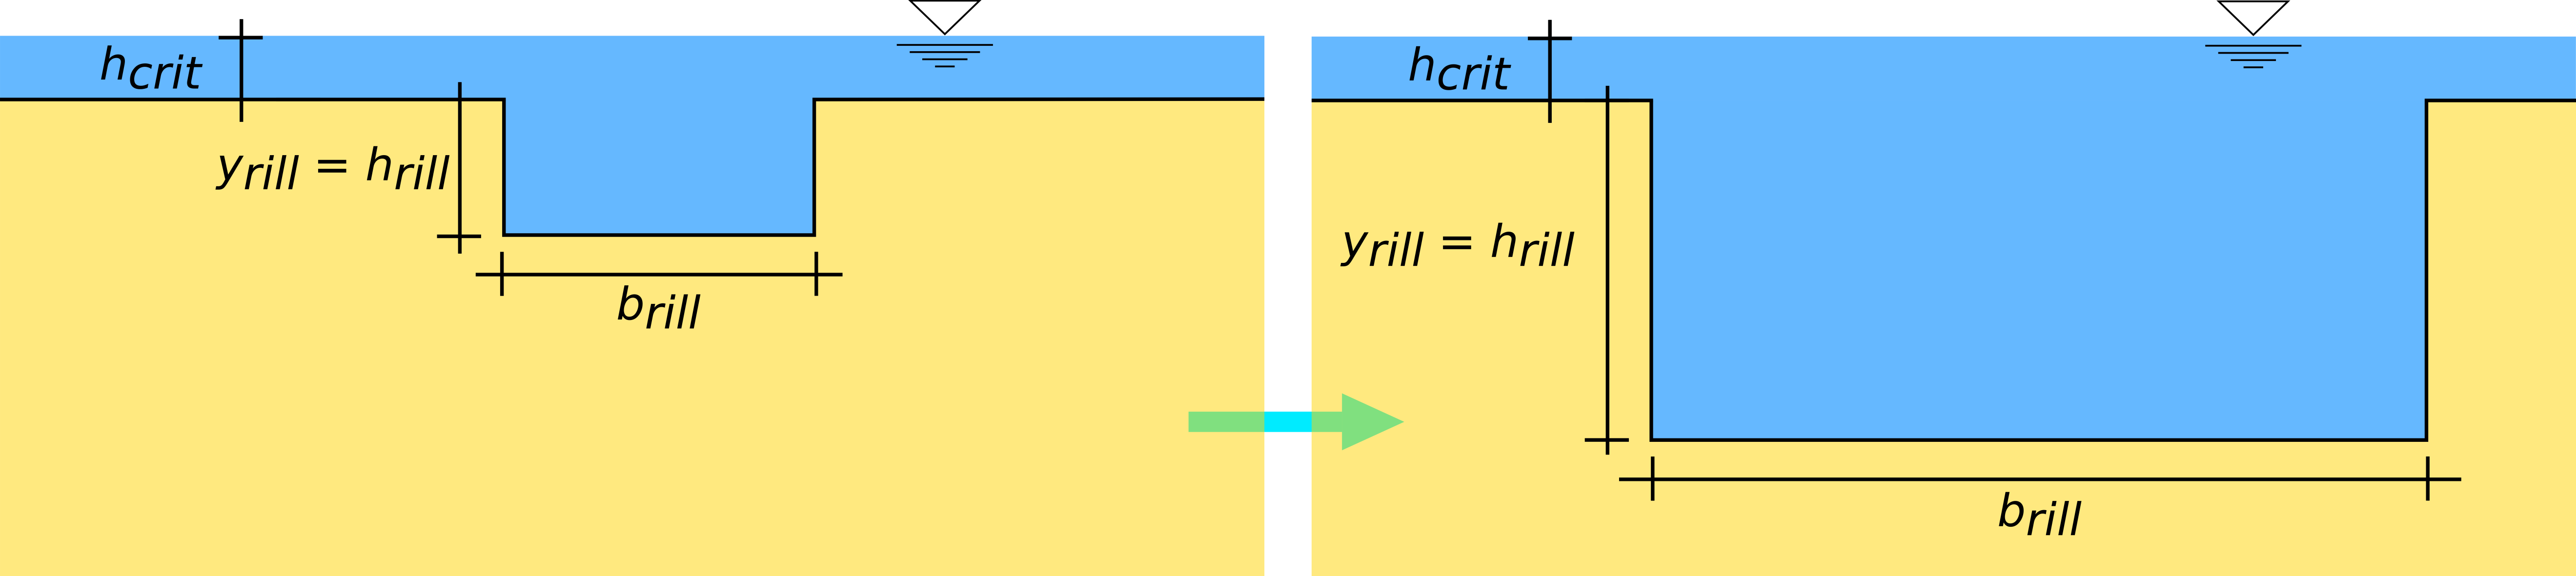
\includegraphics[width=1\linewidth]{./img/rill_schema_plneni.png}
                \caption{Scheme of the rill size during increasing surface runoff.}
                \label{fig:rill_plneni}
            \end{figure}


            During the recession limb of the hydrograph, the rill size “locks”, and
            $h_{rill}$ decreases until the rill is empty. The scheme of the emptying rill
            and the rill flow is shown in Figure~\ref{fig:rill_prazdneni}. In this case,
            $R_{rill}$ is calculated from fixed $b_{rill}$ and decreasing $h_{rill}$.
            $R_{rill}$ for decreasing rill flow is calculated as:
            \begin{equation}
                R_{rill} = \frac{h_{rill}b_{rill}}{2h_{rill}+b_{rill}},
              \label{eq:rrill2}
            \end{equation}
            where:
            \begin{equation}
              b_{rill} = y_{rill}/0.7
              \label{eq:brill2}
            \end{equation}

            \begin{figure}[t]
                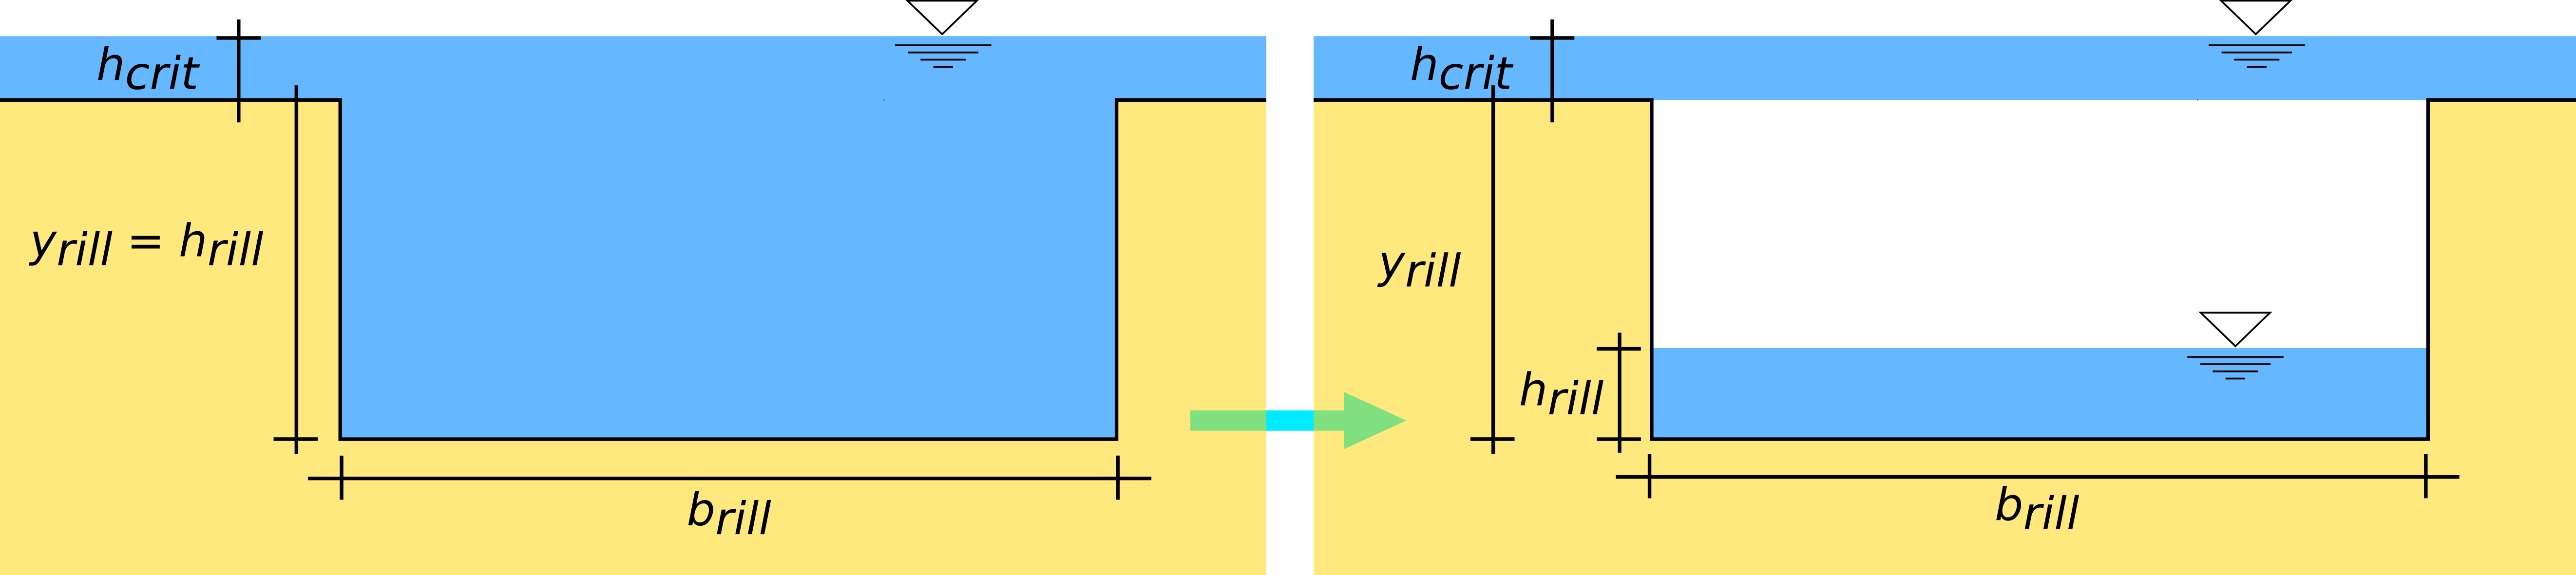
\includegraphics[width=1\linewidth]{./img/rill_schema_prazdneni.png}
                \caption{Scheme of the rill size during the recession limb of the hydrograph.}
                \label{fig:rill_prazdneni}
            \end{figure}

            The total water balance in cell i, where a rill is developed, is calculated as:

            \begin{equation}
                \frac{\mathrm{d}h_i}{\mathrm{d}t} = es_i + q^{in}_{sheet,i}(h_{sheet,i})
                +q^{in}_{rill,i}(h_{rill,i}) - (inf_i + q^{out}_{sheet,i}(h_{sheet,i}) +
                q^{out}_{rill,i}(h_{rill,i}))
                %
                %
                %h_{i,t} =h_{i,t} + \mathrm{d}t (es_{i,t-1} + \sum_j^m q^{out}_{j,t-1}-
                %inf_{i,t-1} - q^{out}_{i,t-1}),
            \end{equation}
            where:
            \begin{equation}
                q^{in}_{sheet,i} = \sum_j^m q^{out}_{sheet, j}(h_{sheet,j}),\quad \mathrm{and}
            \end{equation}
            \begin{equation}
                q^{in}_{rill,i} = \sum_j^m q^{out}_{rill, j}(h_{rill,j})
            \end{equation}

            and:
            \begin{equation}
               h = h_{rill} + h_{sheet}  
            \end{equation}

            The rill water level is recalculated to cover the whole cell and not just the
            bottom of the rill, as shown in Figures \ref{fig:rill_plneni} and
            \ref{fig:rill_prazdneni}.

            %For each soil type a critical value of the tangential stress and velocity was
            %estimated. From this critical value critical height in each cell is calculated.
            %In principle this is a comparison of the current level and its critical value
            %at each time interval. If the critical value is exceeded, the calculation
            %enters the stage at which the rill starts to form. Dimensions of the rills are
            %calculated from volume of the water exceeding the critical value. Sheet surface
            %runoff is then calculated using the critical value level instead of current
            %height in the time step. Once the level has dropped below the critical height
            %value, the calculation returns only in the calculation of surface runoff. The
            %resulting rasters of rill flow and speed in the rill are stored in
            %user-selected directory along with vector shapefile of created rills.
            %Calculation of the flow in the rill is based on Manning equation. 

        \subsubsection{Rill formation (JJ)}

            %The rill flow is also included in the calculation. In SMODERP2D, rill flow in a
            %cell occurs if [Equation], where [Equation] is the critical water level. The
            %water flow corresponding to the water level above the critical water level has
            %enough energy to start to carry the soil particles and to create a rill. 
            %
            %The critical water level [Equation] is calculated as: 
            %
            %[Equation] 
            %	
            %
            %(7) 
            %
            %where [Equation] is the water corresponding to the critical velocity, and
            %[Equation] is the water level corresponding to the critical shear stress. As
            %shown in Formula (7), [Equation] uses several values obtained with a different
            %approach. This approach is adopted in order to remain on the safe side of the
            %emergence of a rill, since [Equation] is more sensitive to the sheet flow
            %velocity and [Equation] is more sensitive to the slope of the soil surface.  
            %
            %When the condition [Equation] is fulfilled, a rill starts to develop in a given
            %cell and [Equation]. In SMODERP2D, the rill is a dynamic component and can
            %increase as the rill flow increases. The rill volume is controlled by the
            %volume of water corresponding to the rill water level [Equation] This volume is
            %calculated as: 
            %
            %[Equation] 
            %	
            %
            %(8) 
            %
            %where: 
            %
            %[Equation] 
            %	
            %
            %(9) 
            %
            %P stands for the size of the raster cell. 

        \subsubsection{Rill hydraulics (JJ)}

            %The rill is simplified as a small channel at the soil surface with a
            %rectangular cross section. The rectangle has width[Equation] and rill height
            %[Equation]. The rill flow is as calculated with the Manning equation:  
            %
            %[Equation] 
            %	
            %
            %(10) 
            %
            %where A is the cross section of the rill, [Equation] is the
            %roughness in the rill, s is the surface slope, and [Equation] is the
            %hydraulic radius of the rill.  
            %
            %As stated above, the size of the rill changes as [Equation] increases. The
            %scheme of this change is shown in Figure 1. The change in the rill flow varies
            %with the change in [Equation] in Equation (10), since [Equation] increases, and
            %therefore [Equation] and [Equation] also increase. The [Equation] for an
            %increasing rill is calculated as: 
            %
            %[Equation] 
            %	
            %
            %(11) 
            %
            %where: 
            %
            %[Equation] 
            %	
            %
            %(12) 
            %
            %  
            %
            %Figure 1. Scheme of the rill size during increasing surface runoff. 
            %
            %During the recession limb of the hydrograph, the rill size
            %“locks”, and [Equation] decreases until the rill is empty. The scheme
            %of the emptying rill and the rill flow is shown in Figure 2. In this
            %case, [Equation] is calculated from fixed [Equation] and decreasing
            %[Equation]. [Equation] for decreasing rill flow is calculated as: 
            %
            %[Equation] 
            %	
            %
            %(13) 
            %
            %where: 
            %
            %[Equation] 
            %	
            %
            %(14) 
            %
            % 
            %
            %Figure 2. Scheme of the rill size during the recession limb of the hydrograph. 
            %
            %The total water balance in cell i, where a rill is developed, is calculated as: 
            %
            %[Equation] 
            %	
            %
            %(15) 
            %
            %where: 
            %
            %[Equation] 
            %	
            %
            %(16) 
            %
            %[Equation] 
            %	
            %
            %(17) 
            %
            % 
            %
            %and: 
            %
            %[Equation] 
            %	
            %
            %(18) 
            %
            % 
            %
            %The rill water level is recalculated to cover the whole cell and not just the bottom of the rill, as shown in Figures 1 and 2. 

 

    \subsection{Kinematic / Diffuse approach}

        \subsubsection{Kinematic}
        \subsubsection{Diffuse}

    \subsection{Implicit /Explicit approach}

        \subsubsection{Implicit}
        \subsubsection{Explicit}

    \subsection{Impute data requirements and description}

        \subsubsection{DMR}
        \subsubsection{Soil}
        \subsubsection{Land Use}
        \subsubsection{Soil and Land Use  combination}

\section{Stream hydrology and hydraulics}

    \subsection{Segmentation}
    \subsection{Kinematic approach - Manning formula}
    \subsection{Stream shape}
    \subsection{Stream characteristics}

\section{Impute data requirements and description}

\section{Output data description}

    \subsection{Basic data}
    \subsection{Hydrograph data}
    \subsection{Control}
    \subsection{Temporary data}

\section{Numerical solution and source code description}

    \subsection{Source code architecture}
    \subsection{NumPy solution}
    \subsection{Implicit method numerical solution}

\section{Reference}




%
%

%


  \FloatBarrier
  %\newpage

  \part*{References}
  \bibliographystyle{agsm}
  \bibliography{bib/bib}

\end{document}


